% (c)~2014 Claudio Carboncini - claudio.carboncini@gmail.com
% (c)~2014 Dimitrios Vrettos - d.vrettos@gmail.com
% (c) 2014 Daniele Zambelli - daniele.zambelli@gmail.com

\chapter{La probabilità}

\section{Gli eventi}
\label{sec:09_eventi}

L'esito del lancio di una moneta o di un dado, l'esito di un'estrazione del 
lotto, il sesso di un nascituro, la durata di una lampadina o di un computer 
sono esempi di fenomeni la cui realizzazione non può essere prevista con 
certezza; per questo vengono detti eventi casuali o aleatori (dal latino alea, 
dado). Spesso è necessario prendere decisioni in condizioni di incertezza: in 
quale università proseguire gli studi, decidere se fare il vaccino contro 
l'influenza, scommettere sulla vincita di una squadra, sull'uscita di una 
sequenza di numeri al gioco del Lotto. E' quindi fondamentale, nei confronti di 
un fenomeno dall'esito incerto, poter identificare quali sono gli eventi che si 
possono verificare ed inoltre riuscire ad esprimere il proprio grado di fiducia 
nel verificarsi di tali eventi.

Quali sono gli eventi possibili per un dato fenomeno aleatorio? Supponiamo di 
lanciare un dado e di essere interessati alla faccia che si presenta dopo aver 
effettuato il lancio. Il lancio del dado rappresenta l'esperimento oggetto del 
nostro studio, l'uscita del numero 4 o l'uscita di un numero dispari sono detti 
\emph{eventi aleatori o casuali}, in quanto sappiamo che si presenterà una 
delle 
facce, ma non sappiamo quale.

\begin{definizione}
Si chiama \emph{evento casuale} il risultato di un \emph{fenomeno aleatorio}.
\end{definizione}

Se si considera la proposizione ``Oggi farà bel tempo'' è evidente che non è 
chiaro cosa si intende per bel tempo (senza pioggia? senza nuvole? con il 
sole?) 
né il luogo a cui ci si riferisce. Sarebbe meglio affermare per esempio 
``Stamani a Milano ci sarà il sole''. È necessario quindi specificare con 
precisione l'evento che si considera in modo da essere sicuri se l'evento si è 
verificato o meno.

Nel lancio di un dado sono possibili sei risultati, espressi dai numeri da 1 a 
6 
e solo uno di essi si realizzerà.

Chiamiamo questi sei risultati \emph{eventi elementari} e indichiamo il loro 
insieme con 
$\Omega:$ 
\[\Omega =\{1,2,3,4,5,6\}.\]

\begin{definizione}
Si chiama \emph{spazio degli eventi}, l'insieme di tutti gli esiti possibili 
del 
fenomeno considerato. Tale insieme viene indicato con $\Omega $.
\end{definizione}

L'insieme $\Omega $ non esaurisce la totalità degli eventi collegati al lancio 
del dado: non comprende per esempio l'evento $P=\{$Numero pari$\}$ o l'evento $M=\{$Numero
minore di $3\}$. Tuttavia~ $\Omega $ permette di rappresentare qualsiasi 
evento come suo particolare sottoinsieme.

\begin{definizione}
Si chiama \emph{evento elementare} ogni elemento dell'insieme $\Omega$, mentre 
\emph{evento composto} un sottoinsieme qualsiasi di $\Omega$.
\end{definizione}

Estraiamo una carta da un mazzo di 52 carte e consideriamo i seguenti eventi: 
uscita di un asso di cuori, uscita di un re. Qual è la differenza fra questi 
due 
eventi? Il primo dei due è un \emph{evento elementare}, mentre l'altro è un 
evento formato da quattro eventi elementari (tutti i possibili re presenti nel 
mazzo) e viene detto \emph{evento composto}.

Sono esempi di eventi composti l'uscita di un numero dispari nel lancio di un 
dado o l'estrazione di due palline rosse da un'urna contenente 3 palline rosse 
e 
7 nere.

Consideriamo ora due eventi che rivestono una particolare importanza: l'uscita 
del 7 nel lancio di un dado e l'uscita di un numero minore di 7 sempre nel 
lancio di un dado. È evidente che l'uscita del 7 non si verificherà mai, mentre 
l'uscita di un numero minore di 7 è sempre verificato.

\begin{definizione}
Chiamiamo \emph{evento impossibile}, e lo indicheremo $\varnothing$, un evento 
che non può verificarsi in alcun caso.
Chiamiamo \emph{evento certo} un evento che accade sicuramente e che è 
costituito dall'insieme di tutti gli eventi elementari di $\Omega $, cioè da 
tutti gli esiti possibili del fenomeno considerato.
\end{definizione}

Gli eventi elementari di un insieme $A$ e gli eventi composti che si possono 
ottenere con gli eventi elementari di $A$ formano lo \emph{spazio degli eventi} 
che viene indicato con $\wp (A)$. In generale infatti, qualunque evento è identificabile con
un elemento dell'insieme delle parti di $\Omega$, ovvero $\wp (\Omega )$ (definito come insieme di
tutti i sottoinsiemi di $\Omega$).
\begin{osservazione}
 Ricordiamo che la cardinalità dell'insieme delle parti cioè il numero degli 
eventi che si possono formare con gli elementi di $\Omega $ è dato da 
$\mathit{card}(\wp (\Omega ))=2^n$, dove $n$ rappresenta il numero degli eventi 
elementari. Così nel lancio del dado abbiamo $2^6=64$ possibili eventi, 
considerando anche l'insieme vuoto $\varnothing $ che rappresenta l'evento 
impossibile e l'insieme $\Omega =\{1,2,3,4,5,6\}$ che rappresenta l'evento 
certo.
\end{osservazione}
\\[9pt]
Gli eventi sono gli oggetti dello studio della probabilità e in genere si 
indicano con le lettere maiuscole $A,B,\ldots $ mentre per le operazioni e le 
relazioni tra eventi si usano i corrispondenti simboli che si sono utilizzati 
per le operazioni e le relazioni tra insiemi. Molto utile è infatti la 
rappresentazione con i diagrammi di Venn (vedi Figura \ref{fig:9.1}).
\begin{inaccessibleblock}[Figura: TODO]
 \begin{figure}[tp]
\begin{minipage}[t]{.45\textwidth}
\centering% (c) 2013 Claudio Carboncini - claudio.carboncini@gmail.com
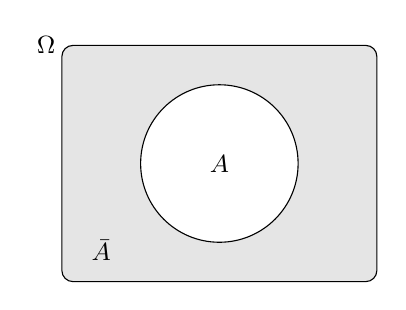
\begin{tikzpicture}[x=10mm,y=10mm,font=\small]
\definecolor{circle area}{gray}{0.9}
\draw[rounded corners, fill=circle area] (0,0) rectangle (4,3) (-.2,3) node {$\Omega$} ;
\node[]  at (.5,.4) {$\bar{A}$};
\draw[fill=white](2,1.5) circle (1) (2,1.5) node {$A$};
\end{tikzpicture}

\caption{La \emph{negazione} di un evento $A$, indicata con $\bar {A}$, è 
l'evento che si verifica quando non si verifica $A$.}\label{fig:9.1}
\end{minipage}\hfil
\begin{minipage}[t]{.45\textwidth}
\centering% (c) 2013 Claudio Carboncini - claudio.carboncini@gmail.com
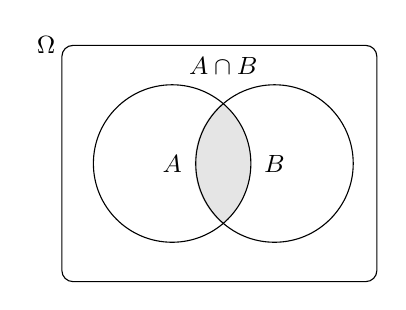
\begin{tikzpicture}[filled/.style={fill=circle area, draw=circle edge, thick},x=10mm,y=10mm,font=\small]
\def\firstcircle{(1.4,1.5) circle (1cm)}
\def\secondcircle{(2.7,1.5) circle (1cm)}

\definecolor{circle edge}{gray}{0.9}
\definecolor{circle area}{gray}{0.9}
    \begin{scope}
        \clip \firstcircle;
        \fill[filled] \secondcircle;
    \end{scope}
    \draw\firstcircle node {$A$};
    \draw \secondcircle node {$B$};
    \node[anchor=south] at (current bounding box.north) {$A \cap B$};
\draw[rounded corners] (0,0) rectangle (4,3) (-.2,3) node {$\Omega$} ;

\end{tikzpicture}

\caption{L'\emph{intersezione} tra gli eventi $A$ e $B$ indicata con $C=A\cap 
B$ 
è l'evento che si verifica quando si verificano sia $A$ che $B$.}
\end{minipage}
\vspace{5px}
\begin{minipage}[t]{.45\textwidth}
\centering% (c) 2013 Claudio Carboncini - claudio.carboncini@gmail.com
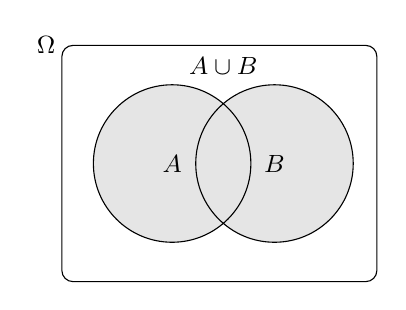
\begin{tikzpicture}[filled/.style={fill=circle area, draw=black, thin},x=10mm,y=10mm,font=\small]

\def\firstcircle{(1.4,1.5) circle (1cm)}
\def\secondcircle{(2.7,1.5) circle (1cm)}

\definecolor{circle area}{gray}{.9}

 \draw[filled] \firstcircle node {$A$}
                  \secondcircle node {$B$};
 \node[anchor=south] at (current bounding box.north) {$A \cup B$};
\draw[rounded corners] (0,0) rectangle (4,3) (-.2,3) node {$\Omega$} ;

\end{tikzpicture}

\caption{L'\emph{unione} tra gli eventi $A$ e $B$ indicata con $C=A\cup B$ è 
l'evento che si verifica quando si verifica almeno uno dei due eventi.}
\end{minipage}\hfil
\begin{minipage}[t]{.45\textwidth}
\centering% (c) 2013 Claudio Carboncini - claudio.carboncini@gmail.com
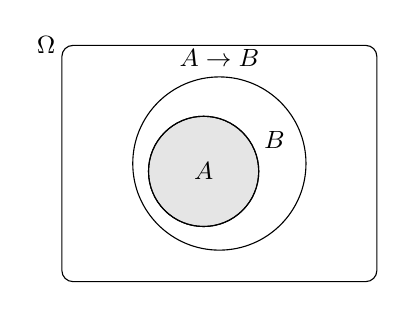
\begin{tikzpicture}[filled/.style={fill=circle area, draw=black, thin},x=10mm,y=10mm,font=\small]
\def\firstcircle{(2,1.5) circle (1.1cm)}
\def\secondcircle{(1.8,1.4) circle (.7cm)}

\definecolor{circle edge}{gray}{0.9}
\definecolor{circle area}{gray}{0.9}
    \begin{scope}
        \clip \firstcircle;
        \fill[filled] \secondcircle;
    \end{scope}
    \draw\firstcircle;
    \node[]  at (2.7,1.8) {$B$}; 
    \draw \secondcircle node {$A$};
    \node[anchor=south] at (current bounding box.north) {$A \to B$};
\draw[rounded corners] (0,0) rectangle (4,3) (-.2,3) node {$\Omega$} ;

\end{tikzpicture}

\caption{L'evento $A$ \emph{implica} l'evento $B$, in simboli $ A \subseteq B$, 
se ogni volta che si verifica $A$ si verifica anche $B$.}
\end{minipage}
\vspace{5px}
\begin{minipage}[t]{.45\textwidth}
\centering% (c) 2013 Claudio Carboncini - claudio.carboncini@gmail.com
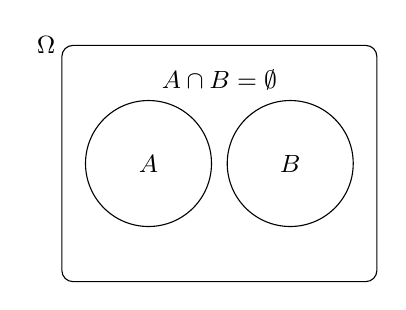
\begin{tikzpicture}[filled/.style={fill=circle area, draw=circle edge, thick},x=10mm,y=10mm,font=\small]
\def\firstcircle{(1.1,1.5) circle (.8cm)}
\def\secondcircle{(2.9,1.5) circle (.8cm)}

\definecolor{circle edge}{gray}{0.8}
\definecolor{circle area}{gray}{0.8}
    \begin{scope}
        \clip \firstcircle;
        \fill[filled] \secondcircle;
    \end{scope}
    \draw\firstcircle node {$A$};
    \draw \secondcircle node {$B$};
    \node[anchor=south] at (current bounding box.north) {$A \cap B=\emptyset$};
\draw[rounded corners] (0,0) rectangle (4,3) (-.2,3) node {$\Omega$} ;

\end{tikzpicture}

\caption{Due eventi $A$ e $B$ si dicono \emph{incompatibili}, se il verificarsi 
dell'uno esclude il verificarsi dell'altro.}
\end{minipage}\hfil
\begin{minipage}[t]{.45\textwidth}
\centering% (c) 2013 Claudio Carboncini - claudio.carboncini@gmail.com
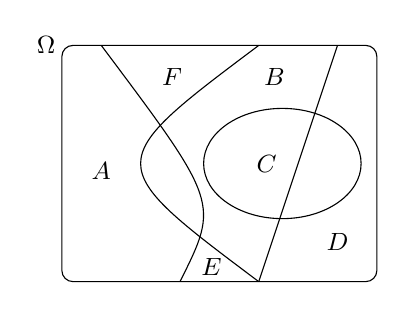
\begin{tikzpicture}[x=10mm,y=10mm,font=\small]
\draw[rounded corners] (0,0) rectangle (4,3) (-.2,3) node {$\Omega$} ;
\draw (.5, 3) .. controls(2,1) .. (1.5, 0);
\node at (.5,1.4) {$A$};
\draw (2.5, 3) .. controls(.5,1.5) .. (2.5, 0);
\node at (2.7,2.6) {$B$};
\draw (2.8,1.5) ellipse (1 and .7);
\node at (2.6,1.5) {$C$};
\draw (3.5,3) -- (2.5,0);
\node at (3.5,.5) {$D$};
\node at (1.9,.18) {$E$};
\node at (1.4,2.6) {$F$};
\end{tikzpicture}

\caption{Due o più eventi si dicono \emph{esaustivi}, se almeno uno di essi si 
verifica. L'unione di tali eventi coincide con l'insieme $\Omega$.}
\end{minipage}
\vspace{5px}
\begin{minipage}[t]{.90\textwidth}
\centering% (c) 2013 Claudio Carboncini - claudio.carboncini@gmail.com
\begin{tikzpicture}[x=10mm,y=10mm,font=\small]
\draw[rounded corners] (0,0) rectangle (4,3) (-.2,3) node {$\Omega$} ;
%insiemi F ed E
\draw [name path=curva1] (.5, 3) .. controls(2,1) .. (1.5, 0);
\draw [color=white, name path=curva2] (2.5, 3) .. controls(.5,1.5) .. (2.5, 0);
\coordinate [name intersections={of=curva1 and curva2, by={a,b}}];
\draw (a) -- (2.5,3);
\draw (b) -- (2.5,0);
%insiemi B ed D
\draw [name path=elipse1] (2.8,1.5) ellipse (1 and .7);
\draw [color=white, name path=linea1] (3.5,3) -- (2.5,0);
\coordinate [name intersections={of=elipse1 and linea1, by={c,d}}];
\draw (c) -- (3.5,3);
\draw (d) -- (2.5,0);

\node at (.5,1.4) {$A$};
\node at (2.7,2.6) {$B_1$};
\node at (2.6,1.5) {$C$};
\node at (3.5,.5) {$D_1$};
\node at (1.9,.18) {$E$};
\node at (1.4,2.6) {$F$};
\end{tikzpicture}

\caption{Un insieme di eventi formato da eventi tra loro incompatibili ed 
esaustivi, genera una partizione nello spazio degli eventi.}
\end{minipage}\hfil
\end{figure}
\end{inaccessibleblock}

\begin{definizione}
Se $ n $ eventi $A,B,\ldots,F$ sono esaustivi (cioè 
$A\,\cup\,B\,\cup\dots \cup \,F=\Omega $) e a due a due incompatibili (ovvero
$A\,\cap\,B=A\,\cap\,C=B\,\cap\,C=\dots=\varnothing$) diremo che essi formano una \emph{partizione dello spazio degli 
eventi}.
\end{definizione}

% \vspazio\ovalbox{\risolvii \ref{ese:9.1}, \ref{ese:9.2}, \ref{ese:9.3}, 
% \ref{ese:9.4}, \ref{ese:9.5}.}

\section{Definizioni di probabilità}
\label{sec:09_definizioni}

Nel linguaggio comune l'uso del termine probabilità è abbastanza chiaro e 
uniforme. Si dice che un certo fatto o evento è più o meno probabile a seconda 
che ci si aspetti che si verifichi più o meno facilmente.

La probabilità è dunque una misura del grado di fiducia associato al 
verificarsi di un evento e dipende dalle informazioni che si hanno a disposizione al 
momento di effettuare la valutazione.

Se diciamo che oggi pioverà con probabilità $0,20=\frac{20}{100}=\frac 1 5$ 
intendiamo che siamo disposti a scommettere 20 centesimi per avere 1 euro nel 
caso che piova e perdere i 20 centesimi della posta nel caso che non piova.
 
\begin{definizione}
La valutazione della probabilità dell'evento $A$ è quel valore $P(A)$ che si 
ottiene dal rapporto tra la quota $q$ che un individuo è disposto 
a pagare per ricevere una vincita $S$ nel caso si verifichi l'evento. Quindi 
$P(A)=\dfrac q S$.
\end{definizione}

Per ottenere una valutazione coerente, per valutare quanto siamo disposti a 
perdere-vincere nella scommessa, dobbiamo immedesimarci nei due ruoli, quello 
dello scommettitore e quello del banco. Inoltre le somme che scommettiamo 
devono 
essere significative per chi procede alla valutazione.
Nessun individuo coerente scommetterebbe su un evento impossibile una quota 
maggiore di 0 qualunque sia la vincita e nessun individuo pagherebbe una 
vincita 
per il verificarsi di un evento certo.
Da queste considerazioni deduciamo che la misura della probabilità appartiene 
all'intervallo $[0,1]$, essendo $ 0 $ il valore che corrisponde all'evento 
impossibile e $1$ quello che corrisponde all'evento certo.

% \begin{postulato}{sulla probabilità}
% 
% La probabilità di un evento E è un numero reale compreso tra 0 e 1: $0\le 
% P(E)\le 1$;
% 
% la probabilità dell'evento impossibile è zero $P(\varnothing )=0$;
% 
% la probabilità dell'evento certo è uguale a uno: $P(\Omega )=1$.
% \end{postulato}
% 
\begin{definizione} La \emph{probabilità} di un evento $P(E)$ è 
un numero reale compreso tra 0 e 1: $0\le 
P(E)\le 1$. In particolare:
\begin{itemize}
 \item[$\quad\circ$]  la probabilità dell'evento impossibile è zero: $P(\varnothing)=0$
 \item[$\quad\circ$] la probabilità dell'evento certo è uguale a uno: $P(\Omega )=1$
\end{itemize}
\end{definizione}

\subsection{La valutazione classica}

La valutazione della probabilità a volte si riconduce a semplici giudizi di 
equiprobabilità: cioè ogni evento elementare dello spazio degli eventi ha la 
stessa probabilità. Così nel lancio di un dado, nel gioco della tombola, nel 
gioco delle carte tutti gli eventi elementari hanno la stessa probabilità. 
Quindi se $n$ sono gli eventi elementari la probabilità di ciascuno di essi è 
$\frac 1 n$.

La probabilità di un evento E è data dal rapporto tra il numero $f$ dei casi 
favorevoli al verificarsi di $E$ e il numero $n$ di tutti i casi possibili, 
purché ugualmente possibili. In simboli: \[ P(E)=\dfrac f n. \]

Mentre nei giochi di sorte si realizzano le condizioni per calcolare tale 
probabilità (conoscenza a priori dei casi possibili, di quelli favorevoli e 
condizione di equiprobabilità) esistono altri eventi casuali per i quali è 
difficile o impossibile calcolare tale probabilità.

% \begin{exrig}
\begin{esempio}
Se in un sacchetto ho 3 palline rosse e 2 palline gialle qual è la probabilità 
che estraendo a caso una pallina questa sia rossa?

La probabilità che si estragga una pallina rossa è $p=\frac 3 
5=0,6=60\text{\%}$, infatti i casi favorevoli al verificarsi dell'evento 
``estrarre una pallina rossa'' sono 3, tante quante sono le palline rosse, i 
casi possibili, tutti ugualmente possibili, sono 5, tante quante palline ci 
sono 
nel sacchetto.
\end{esempio}

\begin{esempio}
Da un mazzo di 40 carte napoletane estraiamo una carta. Calcoliamo la 
probabilità degli eventi:
\begin{itemize*}
\item $A=$ esce una carta di spade;
\item $B=$ esce una carta con il numero 12;
\item $C=$ esce una carta con un numero o una figura;
\item $D=$ esce il sette di denari;
\item $E=$ esce un asso.
\end{itemize*}
I casi possibili sono 40, dato che il mazzo è formato da 40 carte. Anche qui 
siamo in presenza di eventi elementari equiprobabili, applichiamo ancora lo 
schema di valutazione classico
\begin{itemize*}
\item L'evento A è casuale, infatti i casi favorevoli sono 10, dato che il 
mazzo 
ha 10 carte di spade: $P(A)=\frac{10}{40}=\frac 1 4$
\item l'evento B è impossibile dato che non esiste una carta col numero 12: $ 
P(B)=0 $
\item l'evento C è certo, infatti i casi favorevoli sono 40, dato che il mazzo 
ha 12 figure e 28 carte con un numero: $P(C)=1$
\item c'è un solo sette di denari su 40 carte: $P(D)=\frac 1{40}$
\item nel mazzo di 40 carte ci sono 4 assi: $P(E)=\frac 4{40}=\frac 
1{10}=0,1=10\%$
\end{itemize*}
\end{esempio}

\begin{esempio}
Lanciando in aria 3 monete, quale dei seguenti eventi è più probabile?
\begin{itemize*}
\item Ottenere su 3 monete testa;
\item ottenere su 1 moneta testa e su 2 monete croce.
\end{itemize*}
Per rispondere alla domanda occorre calcolare le probabilità dei due eventi. 
Applichiamo la definizione classica. Dobbiamo calcolare tutti gli eventi 
possibili e tutti gli eventi favorevoli.
Aiutiamoci con una tabella per elencare tutti i casi.

\begin{center}
\begin{tabular}{ccc}
prima moneta & seconda moneta & terza moneta\\
\boxT & \boxT & \boxT\\
\boxT & \boxT & \boxC\\
\boxT & \boxC & \boxT\\
\boxT & \boxC & \boxC\\
\boxC & \boxT & \boxT\\
\boxC & \boxT & \boxC\\
\boxC & \boxC & \boxT\\
\boxC & \boxC & \boxC\\
\end{tabular}
\end{center}
I casi possibili sono 8. C'è un solo caso favorevole all'evento ``3 volte 
testa''. La probabilità di questo evento è quindi $p=\frac 1 8=0,125=12,5\%$.

I casi favorevoli all'evento ``1 moneta testa e 2 monete croce'' sono CCT, CTC, 
TCC, quindi 3, allora $p=\frac 3 8=0,375=37,5\%$. Possiamo concludere che 
l'evento più probabile è ottenere 1 testa e 2 croci.
\end{esempio}
% \end{exrig}

\subsection{La valutazione sperimentale}
Se si considera una successione di eventi dello stesso tipo e che avvengono in 
condizioni simili come l'uscita di una determinata faccia in un dado truccato, 
si indica come frequenza relativa $F(E)$ il rapporto tra il numero $v$ dei casi 
in cui si è verificato l'evento e il numero totale delle prove $n$, cioè 
$F(E)=\dfrac v n$.

In una serie di prove ripetute nelle stesse condizioni, la frequenza relativa 
di 
un evento tende a stabilizzarsi intorno a un valore ben preciso al crescere del 
numero delle prove effettuate.
Si assume come valutazione della probabilità dell'evento $E$ il valore intorno 
al quale tende a stabilizzarsi la frequenza relativa dello stesso evento, 
all'aumentare del numero delle prove ripetute alle stesse condizioni: 
$P(E)\approx F(E)=\dfrac v n$.
L'errore che si commette diventa sempre più piccolo al crescere di $n$. La 
valutazione della probabilità così definita si chiama valutazione sperimentale, 
statistica, a posteriori o frequentista.

Anche l'ambito di applicazione di tale valutazione è limitato in quanto 
l'ipotesi che sta alla base della definizione è che l'evento a cui si vuole 
assegnare la probabilità sia pensabile come uno dei possibili risultati di una 
determinata prova e che tale prova sia ripetibile infinite volte nelle stesse 
condizioni.
Si fa molto uso di questo schema di valutazione per stime della probabilità in 
campo economico e sanitario.

% \begin{exrig}
\begin{esempio}
In un'azienda alimentare si producono vasetti di marmellata. In uno studio di 
controllo sono stati evidenziati su 2500 vasetti analizzati 13 con imperfezioni 
e non idonei al commercio. Si valuti la probabilità dell'evento E=``confezioni 
non idonee al commercio''.

Se si considera il campione dei vasetti analizzati significativo rispetto alla 
produzione complessiva delle confezioni prodotte possiamo considerare la 
frequenza relativa dell'evento E come misura della probabilità. Quindi 
$P(E)=F(E)=\frac{13}{2500}=0,0052$.
\end{esempio}

\begin{esempio}
Qual è la probabilità che un certo guidatore faccia un incidente con la 
macchina? Quanto deve pagare, come premio, a una compagnia di assicurazioni in 
modo che, se fa un incidente, la compagnia paghi per intero il danno?

Per rispondere a queste domande le compagnie di assicurazioni sono in grado di 
stimare, sulla base dei numerosissimi incidenti stradali che si verificano ogni 
anno, qual è la probabilità che un guidatore provochi un incidente d'auto.
\end{esempio}

\begin{esempio}
Un sacchetto contiene 10 palline, alcune bianche, altre nere. Si estrae a caso, 
senza guardare nel sacchetto un pallina, si guarda il colore e si rimette il 
sacchetto nella pallina.

Dopo 100 estrazioni abbiamo contato 78 volte la pallina bianca e 22 la pallina 
nera. Possiamo allora ipotizzare che nel sacchetto ci siano 8 palline bianche e 
2 palline nere.
\end{esempio}
% \end{exrig}
\subsection{La valutazione soggettiva}
È la definizione di probabilità che abbiamo dato all'inizio del capitolo: la 
probabilità dell'evento $A$ è quel valore $p$ che l'individuo che procede alla 
valutazione è disposto a pagare per ricevere una vincita unitaria. Se un 
individuo valuta pari $\frac 1 4=25\%$ la probabilità di un certo evento $E$ 
vuol dire che è disposto a pagare $25$ euro a un ipotetico banco per riceverne 
$100$ nel caso che $E$ si verifichi. Naturalmente la scommessa va accettata 
anche come banco che deve essere disposto a scommettere il $75\%=1-p$ sul fatto 
che $E$ non si verifichi: $P(E)=\frac q S$ con $ q=25 $ e $S=100$.
\subsubsection*{Le scommesse}
La definizione soggettiva si applica anche alle scommesse. Supponiamo di 
scommettere sul verificarsi di un evento $E$ a cui attribuiamo probabilità $p$. 
Stabiliamo inoltre di giocare e quindi perdere $q$ euro nel caso l'evento non 
si 
verifichi e di guadagnare $g$ euro nel caso l'evento si verifichi. In genere le 
scommesse si indicano in questo modo: si mette in rapporto la perdita con il 
guadagno $\frac q g$ o anche $q:g$ che si legge $q$ a $g$. In questo caso $q$ e 
$g$ si chiamano le \emph{poste} o le \emph{messe} del gioco.
Che relazione c'è tra questo rapporto e la probabilità?

Se in un grande numero di scommesse così congegnate vincessimo la somma $g$ una 
frazione $p$ di volte e perdessimo la somma $q$ una frazione $1-p$, affinché il 
gioco risulti equo dovremmo avere $p\cdot g-q\cdot (1-p)=0$. Isoliamo $p$ 
nell'uguaglianza:
\begin{equation*}
p\cdot g-q\cdot (1-p)=0 \Rightarrow p\cdot g-q+q\cdot p=0\Rightarrow p\cdot 
(g+q)=q \Rightarrow p=\frac q{g+q}.
\end{equation*}
La relazione è dunque questa: la probabilità di una scommessa $q:g$ è data 
dalla 
perdita q al numeratore e al denominatore la somma complessiva che si incassa 
data dal guadagno più quello che si è scommesso.


% \begin{exrig}
\begin{esempio}
Supponiamo che la vincita ai mondiali di calcio dell'Italia sia data $5:12$ 
cioè 
5 a 12 dai bookmaker inglesi. Quale probabilità assegnano gli allibratori alla 
vincita dell'Italia?

Significa che scommettendo 5 euro sulla vincita dell'Italia ne possiamo vincere 
12 nel caso che l'evento si verifichi.

Quindi la probabilità della vincita dell'Italia sarà:
$P(E)=\frac 5{5+12}=\frac 5{17}=0,294$
\end{esempio}

\begin{esempio}
Leggo sul sito del Corriere della Sera, che per la partita Real 
Madrid-Barcellona, che si giocherà questa sera, la vittoria del Real Madrid 
viene data 1 a 2,60.

Significa che scommettendo 1 euro possiamo vincerne 2,60: la vittoria del Real 
Madrid è stata quindi stimata dal giornale $p=\frac 
1{2,60}=\frac{100}{260}=0,38\ldots$ circa 38\%.
\end{esempio}
% \end{exrig}
% \ovalbox{\risolvii \ref{ese:9.6}, \ref{ese:9.7}, \ref{ese:9.8}, 
%\ref{ese:9.9}, 
% \ref{ese:9.10}, \ref{ese:9.11}, \ref{ese:9.12}, \ref{ese:9.13}, 
%\ref{ese:9.14}, 
% \ref{ese:9.15}, \ref{ese:9.16}, \ref{ese:9.17}, \ref{ese:9.18},}

% \vspazio\ovalbox{\ref{ese:9.19}, \ref{ese:9.20}, \ref{ese:9.21}, 
% \ref{ese:9.22}, \ref{ese:9.23}, \ref{ese:9.24}, \ref{ese:9.25}, 
%\ref{ese:9.26}, 
% \ref{ese:9.27}.}

\section{Probabilità dell'unione di due eventi}
\label{sec:09_unione}

La misura della probabilità si può applicare a tutti gli eventi individuati 
dall'insieme delle parti degli eventi elementari $\wp (\Omega )$. Qualsiasi 
evento si può definire come sottoinsieme dell'insieme elementare (elencando gli 
eventi elementari che ne fanno parte) oppure enunciando una proposizione vera 
nel caso in cui l'evento si verifichi. Possiamo quindi poter esprimere la 
probabilità su eventi composti da due o più eventi di $\wp (\Omega )$ 
attraverso 
le operazioni di unione e intersezione tra insiemi che corrispondono alle 
operazioni di disgiunzione inclusiva e di congiunzione nelle proposizioni.

Per la probabilità dell'evento unione di due eventi occorre distinguere tra 
eventi tra loro incompatibili e eventi tra loro compatibili.

\subsection[Unione di due eventi tra loro incompatibili]{Unione di due eventi 
tra loro incompatibili}

\begin{definizione}
Due eventi A e B si dicono \emph{incompatibili} quando non si possono 
verificare 
contemporaneamente, cioè quando $A\cap B=\varnothing $.
Due eventi A e B si dicono \emph{compatibili} quando si possono verificare 
contemporaneamente, cioè quando $A\cap B\neq \varnothing $.
\end{definizione}

% \begin{exrig}
\begin{esempio}
Nel lancio di un dado regolare calcolare la probabilità dell'uscita del numero 
3 
o di un numero pari.

I due eventi ``$ A= $ Uscita del numero 3'' e ``$ B= $ Uscita di un numero 
pari'' sono eventi incompatibili.

Ci sono due modi per calcolare la probabilità dell'evento unione.
\paragraph{Modo I}: Secondo la valutazione classica la probabilità che esca il 
$3$ o un numero pari è uguale a $\frac 4 6$: infatti i casi favorevoli sono 4 
(le facce 3,2,4,6) su un totale di $6$ casi possibili.
\paragraph{Modo II}: Calcoliamo la probabilità dell'unione dei due eventi 
considerando le proprietà dei singoli eventi. Dato che i due eventi sono 
incompatibili, cioè: $A\cap B=\varnothing $: abbiamo $P(A\cup B)=\frac 1 6+\frac 
3 
6=\frac 4 6$.
\begin{center}
 % (c) 2013 Claudio Carboncini - claudio.carboncini@gmail.com
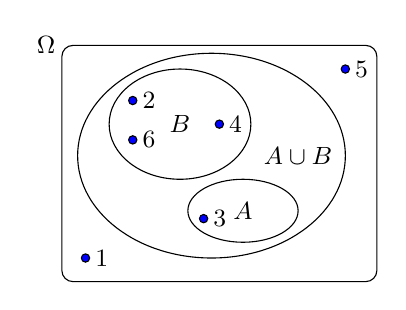
\begin{tikzpicture}[x=10mm,y=10mm,font=\small]
\def\insieme_unione{(1.9,1.6) ellipse (1.7 and 1.3)}
\def\insiemeB{(1.5,2) ellipse (.9 and .7)}
\def\insiemeA{(2.3,.9) ellipse (.7 and .4)}
\draw[rounded corners] (0,0) rectangle (4,3) (-.2,3) node {$\Omega$} ;
\draw\insieme_unione;
\draw\insiemeB node {$B$};
\draw\insiemeA node {$A$};
\draw[fill=blue] (.9,2.3)circle (1.5pt) node[right]{$2$};
\draw[fill=blue] (.9,1.8)circle (1.5pt) node[right]{$6$};
\draw[fill=blue] (2,2)circle (1.5pt) node[right]{$4$};
\draw[fill=blue] (1.8,.8)circle (1.5pt) node[right]{$3$};
\draw[fill=blue] (.3,.3)circle (1.5pt) node[right]{$1$};
\draw[fill=blue] (3.6,2.7)circle (1.5pt) node[right]{$5$};
\node at (3,1.6) {$A \cup B$};
\end{tikzpicture}

\end{center}
\end{esempio}
% \end{exrig}

Possiamo quindi affermare che dati due eventi incompatibili cioè tali che 
$A\cap 
B=\varnothing $ la probabilità dell'evento unione è dato dalla uguaglianza: 
$P(A\cup B)=P(A)+P(B)$.

Può essere utile per avere un'idea intuitiva di questa uguaglianza pensare alla 
probabilità come una massa unitaria distribuita sugli eventi. Se voglio la 
probabilità di $A\cup B$, considero la massa presente su $A$ che addiziono a 
quella presente su $B$.

\subsection{Unione di due eventi tra loro compatibili}

% \begin{exrig}
\begin{esempio}
Consideriamo il lancio di un dado regolare, vogliamo trovare la probabilità 
dell'uscita di un numero maggiore di 2 o di un numero dispari.

Gli eventi ``$ A= $ Uscita di un numero maggiore di 2'' e ``$ B= $ Uscita di un 
numero dispari'' sono compatibili in quanto le facce 5 e 3 appartengono sia 
all'evento $A$ che all'evento $B$.
\begin{center}
 % (c) 2013 Claudio Carboncini - claudio.carboncini@gmail.com
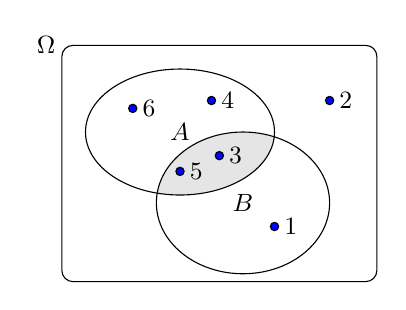
\begin{tikzpicture}[x=10mm,y=10mm,font=\small]

\def\insiemeA{(1.5,1.9) ellipse (1.2 and .8)}
\def\insiemeB{(2.3,1) ellipse (1.1 and .9)}
    \begin{scope}
        \clip \insiemeA;
        \fill[color=gray!20!] \insiemeB;
    \end{scope}
\draw[rounded corners] (0,0) rectangle (4,3) (-.2,3) node {$\Omega$} ;
\draw\insiemeB node {$B$};
\draw\insiemeA node {$A$};
\draw[fill=blue] (.9,2.2)circle (1.5pt) node[right]{$6$};
\draw[fill=blue] (3.4,2.3)circle (1.5pt) node[right]{$2$};
\draw[fill=blue] (1.9,2.3)circle (1.5pt) node[right]{$4$};
\draw[fill=blue] (2.7,.7)circle (1.5pt) node[right]{$1$};
\draw[fill=blue] (2,1.6)circle (1.5pt) node[right]{$3$};
\draw[fill=blue] (1.5,1.4)circle (1.5pt) node[right]{$5$};

\end{tikzpicture}

\end{center}
\paragraph{Modo I}: La probabilità che esca un numero maggiore di $2$ o un 
numero dispari è uguale a $\frac 5 6$: infatti i casi favorevoli sono 5 (le 
facce 1,3,4,5,6) su un totale di $6$ casi possibili.
\paragraph{Modo II}: Calcoliamo la probabilità dell'unione dei due eventi 
considerando le proprietà dei singoli eventi. In questo caso non possiamo 
sommare come nei casi precedenti le probabilità dei singoli eventi. Infatti 
$P(A)+P(B)=\frac 4 6+\frac 3 6=\frac 7 6$ che contraddice l'assioma della 
probabilità. Occorre togliere la probabilità dell'intersezione tra A e B 
contata 
due volte, una volta per A e una per B, che è uguale a $\frac 2 6$: due casi 
favorevoli (le facce 3 e 5) su sei casi possibili: \[P(A\cup 
B)=P(A)+P(B)-P(A\cap B)=\frac 4 6+\frac 3 6-\frac 2 6=\frac 5 6.\]
\end{esempio}

\begin{esempio}
Calcolare la probabilità che estraendo a caso un numero della tombola esso 
contenga la cifra 5 oppure sia multiplo di 5.

La prima domanda da farsi è se i due eventi sono compatibili o incompatibili. 
Poiché esistono numeri della tombola che contengono la cifra 5 e che sono anche 
multipli di 5 (per esempio 15, 50...) i due eventi sono compatibili. Di 
conseguenza bisogna applicare la regola $P(A\cup B)=P(A)+P(B)-P(A\cap B)$.
\begin{itemize*}
\item $ A = $ estrarre un numero che contiene la cifra 5. Questi numeri sono: 
5, 
15, 25, 35, 45, 50, 51, 52, \dots, 59, 65, 75, 85, in tutto 18 ne segue che: 
$p(A)=\frac{18}{90}$
\item $ B = $ estrarre n multiplo di 5. I multipli di 5 sono 5, 10, 15, 20, 
\dots due per ogni decina, quindi 18 in tutto, ne segue che: 
$p(B)=\frac{18}{90}$
\item $A\cap B =$ estrarre un cifra che contiene 5 ed è multiplo di 5. Questi 
numeri sono 5, 15, 25, 35, 45, 50, 55, 65, 75, 85 in tutto sono 10 quindi: 
$p(A\cap B)=\frac{10}{90}$.
\end{itemize*}
Applichiamo la regola della probabilità utilizzata nel modo II del precedente 
esempio quindi:

$A\cup B =$ estrarre un numero che contenga la cifra 5 oppure sia multiplo di 
5. 
\[ P(A\cup B)=P(A)+P(B)-P(A\cap 
B)=\frac{18}{90}+\frac{18}{90}-\frac{10}{90}=\frac{26}{90}\approx 0,29\approx 
29\%. \]
\end{esempio}
% \end{exrig}

Dagli esempi svolti possiamo enunciare il seguente teorema:

\begin{teorema}[delle probabilità totali]
Dati due eventi A e B, entrambi appartenenti allo stesso spazio degli eventi, 
la 
probabilità dell'unione degli eventi è uguale alla somma delle probabilità dei 
singoli eventi meno la probabilità della loro intersezione.
In simboli: \[ P(A\cup B)=P(A)+P(B)-P(A\cap B). \]
\end{teorema}
Se pensiamo alla probabilità come una massa unitaria distribuita sugli eventi, 
per calcolare la probabilità di $A\cup B$, considero la massa presente su A che 
addiziono a quella presente su B a cui devo togliere la massa presente su 
$A\cap 
B$ che è stata contata due volte.

\osservazione Il teorema delle probabilità totali vale anche nel caso degli 
eventi incompatibili. In questo caso $P(A\cap B)=0$ e l'uguaglianza diventa $P(A\cup B)=P(A)+P(B)$.

% \vspazio\ovalbox{\risolvii \ref{ese:9.6}, \ref{ese:9.7}, \ref{ese:9.28}, 
% \ref{ese:9.29}, \ref{ese:9.30}, \ref{ese:9.31}, \ref{ese:9.32}, 
% \ref{ese:9.33}, 
% \ref{ese:9.34}, \ref{ese:9.35}, \ref{ese:9.36}, \ref{ese:9.37} 
% \ref{ese:9.38}.}

\section{Probabilità dell'evento complementare}
\label{sec:09_complementare}

Dato un evento $A$ si definisce \emph{evento complementare} di $A$ indicato con 
$\overline A$ l'evento che si verifica quando non si verifica $A$.
\begin{teorema}[dell'evento complementare]
Dato un evento $E$, la probabilità dell'evento complementare $\overline E$ è 
data da $1$ meno la probabilità dell'evento $E$. In simboli: \[ P(\overline 
E)=1-P(E). \]
\end{teorema}
\begin{proof} per l'assioma introdotto all'inizio del capitolo: \[ P(\overline 
E\cup P(E))=P(\Omega )=1; \]
per il teorema delle probabilità totali essendo i due eventi incompatibili: \[ 
(P(\overline E)\cup P(E))=P(\overline E)+P(E); \]
per la proprietà transitiva dell'uguaglianza: \[ P(\overline E)+P(E)=1 
\Rightarrow P(\overline E)=1-P(E). \]
\end{proof}

Se pensiamo all'analogia della una massa unitaria distribuita sugli eventi, la 
probabilità dell'evento $\overline E$ sarà data dalla massa unitaria meno la 
probabilità di $E$.

% \begin{exrig}
\begin{esempio}
Nel lancio di un dado regolare determina la probabilità che la somma delle 
facce 
non sia uguale a 5.

Consideriamo la probabilità che in un lancio di due dadi si abbia un punteggio 
uguale a 5. I casi possibili sono 36 (ogni faccia del primo dado si può 
associare con ognuna delle 6 facce del secondo dado), mentre i casi favorevoli 
all'evento sono 4, precisamente (1,4), (4,1), (2,3) e (3,2). Quindi $P(E)=\frac 
4{36}=\frac 1 9$.

Per conoscere la probabilità dell'evento complementare cioè la probabilità che 
la somma delle due facce del dado non sia uguale a 5, risulterebbe piuttosto 
laborioso trovare tutti i casi in cui la somma delle due facce sia uguale a 2, 
3, 4, 6, 7, 8, 9, 10, 11 e 12, si può invece applicare la regola $P(\overline 
E)=1-P(E)$ cioè nel nostro caso $P(\overline E)=1-P(E)=1-\frac 1 9=\frac 8 9$.
\end{esempio}
% \end{exrig}

\osservazione L'uguaglianza sulla probabilità dell'evento complementare può 
risultare molto utile nel risolvere alcuni problemi. A volte è più facile o 
indispensabile calcolare la probabilità dell'evento complementare che calcolare 
direttamente la probabilità dell'evento.

% \vspazio\ovalbox{\risolvii \ref{ese:9.39}, \ref{ese:9.40}, \ref{ese:9.41}, 
% \ref{ese:9.42}, \ref{ese:9.43}, \ref{ese:9.44}, \ref{ese:9.45}, 
% \ref{ese:9.46}.}

\section{La probabilità dell'evento intersezione di due eventi}
\label{sec:09_intersezione}

Dati due eventi $A,B\in \wp (\Omega )$ ci proponiamo di calcolare la 
probabilità 
dell'evento intersezione cioè $P(A\cap B)$, partendo dalla probabilità dei singoli
eventi $ P(A) $ e $ P(B) $. Si tratta quindi di stimare con quale 
probabilità i due eventi avvengono congiuntamente. Occorre innanzitutto 
verificare che i due eventi non siano incompatibili in quanto in questo caso 
l'evento intersezione è impossibile.

Per la probabilità dell'intersezione di due eventi occorre distinguere tra 
eventi tra loro \emph{indipendenti} e eventi tra loro \emph{dipendenti}.

\subsection{Intersezione di due eventi tra loro indipendenti}

Due eventi A e B si dicono \emph{indipendenti} se il verificarsi di A \emph{non 
cambia} la probabilità del verificarsi di B, si dicono invece \emph{dipendenti} 
se il verificarsi di A \emph{cambia} la probabilità di B rispetto a quella 
valutata per B prima del verificarsi di A.
% \newpage
% \begin{exrig}
\begin{esempio}
Determinare la probabilità che lanciando una moneta e un dado regolari esca 
testa e un numero maggiore di 4.
\begin{itemize}
\item $ A = $ Uscita di Testa nel lancio di una moneta $\to P(A)=\frac 1 2$
\item $ B = $ Uscita di un numero maggiore di 4 nel lancio di un dado $\to 
P(B)=\frac 2 6$
\item $(A\cap B)$= Uscita di testa e di un numero maggiore di 4 nel lancio di 
una moneta e di un dado.
\end{itemize}
Vediamo come determinare $P(A\cap B)$.
I due eventi A e B non si influenzano in quanto l'uscita di testa non modifica 
la probabilità dell'uscita di 4 nel lancio del dado.

Notiamo subito una situazione diversa rispetto a quella precedente dell'unione 
di due eventi. Nel caso precedente, lo spazio degli eventi era lo stesso per 
l'evento A, per l'evento B e per l'evento unione $A\cup B$.
Mentre, per l'evento A, l'insieme degli eventi elementari è $\Omega 
_1=\{T,C\}$, per l'evento B invece l'insieme degli eventi elementari è $\Omega 
_2=\{1,2,3,4,5,6\}$. L'evento $(A\cap B)$ ha il seguente insieme degli eventi 
elementari: \[ \Omega 
=\{(T,1);(T,2);(T,3);(T,4);(T,5);(T,6);(C,1);(C,2);(C,3);(C,4);(C,5);(C,6)\}. \]

Lo spazio degli eventi elementari dell'intersezione è dato dal prodotto 
cartesiano dello spazio elementare di A moltiplicato per quello di B. Si può 
calcolare la probabilità in due modi:
\paragraph{Modo I}: Si indicano i casi favorevoli e i casi possibili rispetto 
all'evento intersezione: i casi favorevoli all'evento sono due: $(A\cap 
B)=\{(T,5);(T,6)\}$, i casi possibili sono dodici: \[\Omega 
=\{(T,1);(T,2);(T,3);(T,4);(T,5);(T,6);(C,1);(C,2);(C,3);(C,4);(C,5);(C,6)\} \] 
la probabilità dell'evento intersezione è: $P(A\cap B)=\frac 2{12}=\frac 1 6$.

\begin{center}
 % (c) 2013 Claudio Carboncini - claudio.carboncini@gmail.com
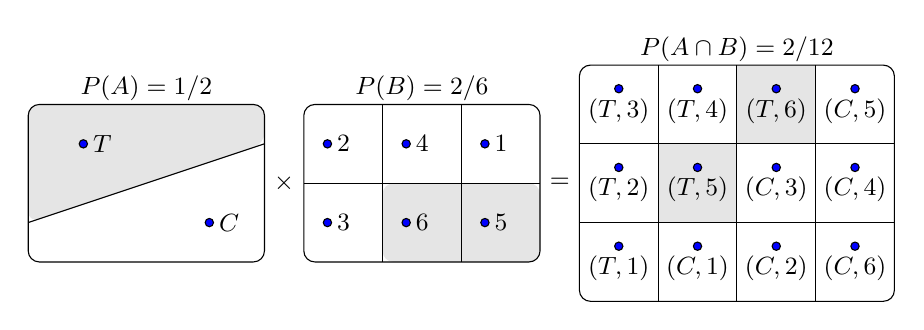
\begin{tikzpicture}[x=10mm,y=10mm,font=\small]

\def\rettangolo{-- ++(3,0) -- ++(0,2) -- ++(-3,0) -- cycle}
\def\insieme_int{-- ++(4,0) -- ++(0,3) -- ++(-4,0) -- cycle}
 %insieme1
\fill[rounded corners, color=gray!20!] (0,.5) -- (0,2) -- (3,2) -- (3,1.5) -- cycle;
\draw[rounded corners] (0,0) \rettangolo;
\node at (1.5,2.2) {$P(A)=1/2$};
\draw (0,.5) -- (3,1.5);
\draw[fill=blue] (.7,1.5) circle (1.5pt) node[right] {$T$};
\draw[fill=blue] (2.3,.5) circle (1.5pt) node[right] {$C$};
%insieme 2
\fill[rounded corners, color=gray!20!] (4.5,0) -- (6.5,0) -- (6.5,1) -- (4.5,1) -- cycle;
\draw[rounded corners] (3.5,0) \rettangolo;
\draw (3.5,1) -- (6.5,1);
\foreach \x in {4.5,5.5}{
\draw (\x,0)--(\x,2);
\draw (\x,0)--(\x,2);}
\foreach \x in {3.8,4.8,5.8}
   \foreach \y in {0.5,1.5}
   { \draw[fill=blue] (\x,\y) circle (1.5pt);}
\draw node[right] at (3.8,1.5) {$2$};
\draw node[right] at (4.8,1.5) {$4$};
\draw node[right] at (5.8,1.5) {$1$};

\draw node[right] at (3.8,0.5) {$3$};
\draw node[right] at (4.8,0.5) {$6$};
\draw node[right] at (5.8,0.5) {$5$};
\node at (5,2.2) {$P(B)=2/6$};
\node at (3.25,1) {$\times$};
%insieme risultato
\fill[color=gray!20!] (8,.5) -- (8,1.5) -- (9,1.5) -- (9,.5) -- cycle;
\fill[color=gray!20!] (9,1.5) -- (9,2.5) -- (10,2.5) -- (10,1.5) -- cycle;
\draw[rounded corners] (7,-.5) \insieme_int;
\node at (9,2.7) {$P(A \cap B )=2/12$};
\node at (6.75,1) {$=$};
\foreach \x in {8,9,10}{
\draw (\x,-.5)--(\x,2.5);
\draw (\x,-.5)--(\x,2.5);
\draw (\x,-.5)--(\x,2.5);}
\foreach \y in {.5,1.5}{
\draw (7,\y)--(11,\y);
\draw (7,\y)--(11,\y);}

\foreach \x in {7.5,8.5,9.5,10.5}
   \foreach \y in {0.2,1.2,2.2}
   { \draw[fill=blue] (\x,\y) circle (1.5pt);}
\draw node[below] at (7.5,0.2) {$(T,1)$};
\draw node[below] at (8.5,0.2) {$(C,1)$};
\draw node[below] at (9.5,0.2) {$(C,2)$};
\draw node[below] at (10.5,0.2) {$(C,6)$};

\draw node[below] at (7.5,1.2) {$(T,2)$};
\draw node[below] at (8.5,1.2) {$(T,5)$};
\draw node[below] at (9.5,1.2) {$(C,3)$};
\draw node[below] at (10.5,1.2) {$(C,4)$};

\draw node[below] at (7.5,2.2) {$(T,3)$};
\draw node[below] at (8.5,2.2) {$(T,4)$};
\draw node[below] at (9.5,2.2) {$(T,6)$};
\draw node[below] at (10.5,2.2) {$(C,5)$};

\end{tikzpicture}

\end{center}

\paragraph{Modo II}: Dato che i due eventi non si influenzano, supponiamo di 
procedere con due scelte successive: prima il lancio della moneta con 
probabilità pari a $\frac 1 2$ e poi il lancio del dado con probabilità pari a 
$\frac 2 6$. Se si verifica il primo evento la probabilità si riduce da 1 a 
$\frac 1 2$ a cui devo applicare la probabilità che si verifichi il secondo 
evento pari a $\frac 2 6$, moltiplicando le probabilità dei singoli eventi.
\begin{itemize*}
\item $ A = $ Uscita di Testa nel lancio di una moneta $\to P(A)=\frac 1 2$
\item $ B = $ Uscita di un numero maggiore di 4 nel lancio di un dado $\to 
P(B)=\frac 2 6$
\item $(A\cap B)$= Uscita di testa e di un numero maggiore di 4 nel lancio di 
una moneta e di un dado $\to P(A\cap B)=P(A)\cdot P(B)=\frac 1 2\cdot \frac 2 
6=\frac 2{12}$.
\end{itemize*}
\end{esempio}
% \end{exrig}

\begin{teorema}[(eventi indipendenti)]
Dati due eventi aleatori A e B tra loro indipendenti la 
probabilità dell'evento intersezione tra A e B è data dalla probabilità di A 
moltiplicata per la probabilità di B: \[P(A\cap B)=P(A)\cdot P(B)\]
\end{teorema}

\subsubsection*{Diagrammi ad albero}
Una rappresentazione grafica che può risultare utile nello studio della 
probabilità dell'evento intersezione detto anche studio delle \emph{probabilità 
composte} è il diagramma ad albero. Le linee dell'albero si dicono \emph{rami}, 
mentre i punti da cui partono e arrivano i rami si dicono \emph{nodi,} il nodo 
iniziale si chiama \emph{radice}.

La costruzione di un diagramma ad albero nel caso delle probabilità composte 
consente di eseguire un'analisi completa di tutti i possibili esiti di una 
prova. Ogni percorso dell'albero che va dalla radice al nodo terminale indica 
una sequenza di eventi congiunti, incompatibile con qualsiasi altro percorso 
dell'albero. La probabilità di ogni singolo evento si indica sui rami e 
moltiplicando le probabilità che si incontrano nel percorso si ottiene la 
probabilità della congiunzione degli eventi che formano il percorso. Dato che 
ogni percorso che va dalla radice al nodo terminale individua eventi 
incompatibili, se vogliamo trovare l'unione di due o più percorsi possiamo 
semplicemente sommarli.
L'esempio precedente può essere schematizzato in questo modo:
\begin{center}
 % (c) 2012 Dimitrios Vrettos - d.vrettos@gmail.com
\begin{tikzpicture}[x=10mm,y=10mm,font=\small]
\node [circle, draw] (a) {$\bullet$};
\node [circle, draw, fill=orange!20!] (t) [above right=of a] {$T$};
\node [circle, draw] (c) [below right=of a] {$C$};
\node [rectangle, draw] (d1) at(45:5.5) {$1$};
\node [right=.1 of d1]{$P(T \cap 1)=1/12$};
\node [rectangle, draw] (d2) [below =.2 of d1] {$2$};
\node [right=.1 of d2]{$P(T \cap 2)=1/12$};
\node [rectangle, draw] (d3) [below =.2 of d2] {$3$};
\node [right=.1 of d3]{$P(T \cap 3)=1/12$};
\node [rectangle, draw] (d4) [below =.2 of d3] {$4$};
\node [right=.1 of d4]{$P(T \cap 4)=1/12$};
\node [rectangle, draw, fill=orange!20!] (d5) [below =.2 of d4] {$5$};
\node [right=.1 of d5] (ad1){$P(T \cap 5)=1/12$};
\node [rectangle, draw, fill=orange!20!] (d6) [below =.2 of d5] {$6$};
\node [right=.1 of d6] (ad2){$P(T \cap 6)=1/12$};
\draw (6.7,.55) -- (7.2,.55) -- (7.2,1.2) -- (6.7,1.2);
\node at (7.4,.9) {$+$};
\node [rectangle, draw] (d11) [below =.2 of d6] {$1$};
\node [right=.1 of d11]{$P(C \cap 1)=1/12$};
\node [rectangle, draw] (d22) [below =.2 of d11] {$2$};
\node [right=.1 of d22]{$P(C \cap 2)=1/12$};
\node [rectangle, draw] (d33) [below =.2 of d22] {$3$};
\node [right=.1 of d33]{$P(C \cap 3)=1/12$};
\node [rectangle, draw] (d44) [below =.2 of d33] {$4$};
\node [right=.1 of d44]{$P(C \cap 4)=1/12$};
\node [rectangle, draw] (d55) [below =.2 of d44] {$5$};
\node [right=.1 of d55]{$P(C \cap 5)=1/12$};
\node [rectangle, draw] (d66) [below =.2 of d55] {$6$};
\node [right=.1 of d66]{$P(C \cap 6)=1/12$};

\draw[ultra thick,color=Maroon] (a) -- (t) node[midway,sloped,above] {$1/2$};
\draw (a) -- (c)node[midway,sloped,above] {$1/2$};
\draw (t) -- (d1)node[midway,sloped] {$1/6$};
\draw (t) -- (d2)node[midway,sloped] {$1/6$};
\draw (t) -- (d3)node[midway,sloped] {$1/6$};
\draw (t) -- (d4)node[midway,sloped] {$1/6$};
\draw[thick,color=Maroon] (t) -- (d5)node[midway,sloped] {$1/6$};
\draw[thick,color=Maroon] (t) -- (d6)node[midway,sloped] {$1/6$};
\draw (c) -- (d11)node[midway,sloped] {$1/6$};
\draw (c) -- (d22)node[midway,sloped] {$1/6$};
\draw (c) -- (d33)node[midway,sloped] {$1/6$};
\draw (c) -- (d44)node[midway,sloped] {$1/6$};
\draw (c) -- (d55)node[midway,sloped] {$1/6$};
\draw (c) -- (d66)node[midway,sloped] {$1/6$};

\end{tikzpicture}

\end{center}
L'albero può essere semplificato considerando gli eventi coinvolti e i loro 
complementari.

% \begin{exrig}
\begin{esempio}
In un'urna abbiamo tre palline bianche e due nere. Facciamo due estrazioni 
rimettendo dopo la prima estrazione la pallina nell'urna. Vogliamo calcolare la 
probabilità dell'uscita di una pallina nera nelle due estrazioni.
\begin{itemize*}
\item $ B_{1}= $ nella prima estrazione pallina bianca $\to P(B_1)=\frac 3 5$
\item $ B_{2}= $ nella seconda estrazione pallina bianca $\to P(B_2)=\frac 3 5$ 
in quanto la pallina si rimette nell'urna;
\item $ N_{1}= $ nella prima estrazione pallina nera $\to P(N_1)=\frac 2 5$
\item $ N_{2}= $ nella seconda estrazione pallina nera $\to P(N_2)=\frac 2 5$.
\end{itemize*}
Il problema è sempre lo stesso: calcolare una probabilità su un insieme 
intersezione partendo dalle probabilità degli eventi componenti. Devo 
moltiplicare la probabilità di avere nera nella prima estrazione $P(N_1)=\frac 
2 
5$ con la probabilità di avere nera nella seconda estrazione $P(N_2)=\frac 2 5$ 
in quanto l'uscita della prima pallina nera, evento considerato ora come 
avvenuto, non influenza la probabilità di avere nera alla seconda estrazione in 
quanto la pallina estratta viene rimessa nell'urna. Quindi: $P(N_1\cap 
N_2)=\frac 2 5\cdot \frac 2 5=\frac 4{25}$ in quanto i due eventi sono 
indipendenti.
\begin{center}
 % (c) 2013 Claudio Carboncini - claudio.carboncini@gmail.com
\begin{tikzpicture}[x=10mm,y=10mm,font=\small]

\filldraw[fill=gray!20!, draw=black]
(.7,-1)--(.7,1)--(.9,1)--(.9,-.8)--(3,-.8)--(3,1)--(3.2,1)--(3.2,-1)-- cycle;
\filldraw[fill=black, draw=black]  (1.2,.5) circle (4pt);
\filldraw[fill=black, draw=black]  (2.5,-.3) circle (4pt);
\filldraw[fill=white, draw=black]  (1.4,0) circle (4pt);
\filldraw[fill=white, draw=black]  (2.4,.4) circle (4pt);
\filldraw[fill=white, draw=black]  (1.9,-.5) circle (4pt);

\node [circle, draw] (a) at (5,0) {$\bullet$};
\node [circle, draw] (b1) [above right=of a] {$B_1$};
\node [circle, draw, fill=orange!20!] (n1) [below right=of a] {$N_1$};
\node [circle, draw] (b2) at(15:9) {$B_2$};
\node [right=.1 of b2] {$P(B_1 \cap B_2)=9/25$};
\node [circle, draw] (n2) [below =.7 of b2] {$N_2$};
\node [right=.1 of n2] {$P(B_1 \cap N_2)=6/25$};
\node [circle, draw] (b3) [below =.7 of n2] {$B_2$};
\node [right=.1 of b3] {$P(N_1 \cap B_2)=6/25$};
\node [circle, draw, fill=orange!20!] (n3) [below =.7 of b3] {$N_2$};
\node [right=.1 of n3] {$P(N_1 \cap N_2)=4/25$};
\draw (a) -- (b1)node[midway,sloped,above] {$3/5$};
\draw[ultra thick,color=Maroon] (a) -- (n1) node[midway,sloped,above] {$2/5$};
\draw (b1) -- (b2)node[midway,sloped,above] {$3/5$};
\draw (b1) -- (n2)node[midway,sloped,above] {$2/5$};
\draw (n1) -- (b3)node[midway,sloped,above] {$3/5$};
\draw[thick,color=Maroon] (n1) -- (n3) node[midway,sloped,above] {$2/5$};

\end{tikzpicture}

\end{center}
Le domande che posso fare su questo esperimento sono relative allo spazio degli 
eventi $\wp (\Omega ).$ ove $\Omega 
=\{(B_{1,}B_2);(B_{1,}N_2);(N_{1,}B_2);(N_{1,}N_2)\}$ sono del tipo ``Quale è 
la 
probabilità che escano palline di diverso colore'', ``Qual è la probabilità che 
la prima pallina sia bianca'', ecc.
\end{esempio}
% \end{exrig}

\subsubsection*{Il problema del Cavalier de Méré}
Il Cavalier de Méré pose al grande matematico francese Blaise Pascal nel 1654 
il 
seguente problema.
\begin{problema}
Perché scommettendo alla pari sull'evento $ A= $ ``ottenere almeno una volta un 
6 in 4 lanci di un dado'' ho accumulato una fortuna, mentre rischio la rovina 
scommettendo alla pari sull'evento $ B= $ ``ottenere almeno una coppia di 6 in 
24 lanci di due dadi''.
\end{problema}
Scommettere alla pari 1:1 significa assegnare alla probabilità degli eventi A e 
B il valore pari a $\frac 1 2$.
Consideriamo la probabilità dell'evento A composto dai quattro eventi 
indipendenti ma non incompatibili
\begin{itemize*}
\item $ E_1= $ ottenere 6 nel primo lancio;
\item $ E_{2}= $ ottenere 6 nel secondo lancio;
\item $ E_{3}= $ ottenere 6 nel terzo lancio;
\item $ E_{4}= $ ottenere 6 nel quarto lancio.
\end{itemize*}
In questo caso conviene calcolare la probabilità dell'evento complementare: 
$\overline A=$ non ottenere un 6 in quattro lanci di un dado.
$\overline A=(\overline{E_1}\cap \overline{E_2}\cap \overline{E_3}\cap 
\overline{E_4})$.

Dato che gli eventi sono indipendenti e equiprobabili abbiamo: \[ 
P(\overline{E_1})=P(\overline{E_2})=P(\overline{E_3})=P(\overline{E_4})=\frac 5 
6. \]
I valori di ciascun evento vanno moltiplicati tra loro per la regola vista in 
precedenza. Quindi $P(\overline A)=\frac 5 6\cdot \frac 5 6\cdot \frac 5 6\cdot 
\frac 5 6=\frac{625}{1296}=0,482$.
La probabilità dell'evento A sarà quindi superiore a 0,5 in quanto 
$P(A)=1-P(\overline A)=1-0,482=0,518$ e in un numero considerevole di scommesse 
il Cavalier de Méré accumulava una fortuna.

Consideriamo ora la probabilità dell'evento B, dove valgono considerazioni 
analoghe. Anche in questo caso conviene calcolare la probabilità dell'evento 
complementare $\overline B$. Dato che i casi possibili nel lancio di due dadi 
sono 36 il caso favorevole all'evento 6 nel primo dado e 6 nel secondo dado è 
uno soltanto. Se $P(B)=\frac 1{36} \Rightarrow p(\overline 
B)=1-P(B)=\frac{35}{36}$. Dato che i lanci dei due dadi sono 24 e tutti tra 
loro 
indipendenti avremo:
 \[ p(\overline 
B)=\underbrace{\frac{35}{36}\cdot\frac{35}{36}\cdot\frac{35}{36}
\cdot\ldots\cdot\frac{35}{36}}_{24\text{ volte}}=\frac{35^{24}}{36^{24}}=0,509 
\]
 da cui $P(B)=1-0,509=0,491$. Così è spiegato come mai in un grande numero di 
scommesse scommettendo alla pari il Cavalier de Méré si rovinasse.

% \vspazio\ovalbox{\risolvii \ref{ese:9.47}, \ref{ese:9.48}, \ref{ese:9.49}, 
% \ref{ese:9.50}, \ref{ese:9.51}, \ref{ese:9.52}, \ref{ese:9.53}, 
% \ref{ese:9.54}, 
% \ref{ese:9.55}, \ref{ese:9.56}, \ref{ese:9.57}, \ref{ese:9.58}, 
% \ref{ese:9.59}.}

\subsection{Intersezione di due eventi tra loro dipendenti}
\begin{definizione}
Si chiama \emph{probabilità condizionata} di un evento B rispetto a un evento 
A, la probabilità di B nell'ipotesi che l'evento A si sia già verificato. 
La probabilità di B subordinata o condizionata ad A si indica con $P(B/A)$.
\end{definizione}

% \begin{exrig}
\begin{esempio}
Calcolare la probabilità di avere due palline nere in due estrazioni in un'urna 
contenente tre palline bianche e due nere, questa volta però senza rimettere la 
pallina nell'urna.

Dato che vogliamo calcolare la probabilità dell'evento intersezione $(N_1\cap 
N_2)$ questa sarà data dalla probabilità dell'evento $N_1$ moltiplicata per la 
probabilità dell'evento $N_2$ dopo che si è verificato l'evento $N_1$. La 
probabilità dell'evento $N_2$ dopo il verificarsi di $N_1$ non è la stessa 
dell'esperimento precedente in quanto la pallina estratta non viene rimessa 
nell'urna.
\begin{itemize*}
\item $ N_{1}= $ nella prima estrazione pallina nera $\to P(N_1)=\frac 2 5$
\item$ N_{2}= $ nella seconda estrazione pallina nera, dopo che l'evento $N_1$ 
si è verificato $\to P(N_2/N_1)=\frac 1 4$.
\end{itemize*}
% \newpage
\begin{center}
 % (c) 2013 Claudio Carboncini - claudio.carboncini@gmail.com
\begin{tikzpicture}[x=10mm,y=10mm,font=\small]
\filldraw[fill=gray!20!, draw=black]
(-1,-1)--(-1,.8)--(-.8,.8)--(-.8,-.8)--(.8,-.8)--(.8,.8)--(1,.8)--(1,-1)-- cycle;
\filldraw[fill=black, draw=black]  (-.5,.5) circle (4pt);
\filldraw[fill=black, draw=black]  (-.4,-.4) circle (4pt);
\filldraw[fill=white, draw=black]  (-.2,0) circle (4pt);
\filldraw[fill=white, draw=black]  (.4,.4) circle (4pt);
\filldraw[fill=white, draw=black]  (.2,-.5) circle (4pt);
\node at(0,1) {$P(N_1)=2/5$};

\filldraw[fill=gray!20!, draw=black]
(2,-1)--(2,.8)--(2.2,.8)--(2.2,-.8)--(3.8,-.8)--(3.8,.8)--(4,.8)--(4,-1)-- cycle;
\filldraw[fill=black, draw=black]  (2.6,-.4) circle (4pt);
\filldraw[fill=white, draw=black]  (2.8,0) circle (4pt);
\filldraw[fill=white, draw=black]  (3.4,.4) circle (4pt);
\filldraw[fill=white, draw=black]  (3.2,-.5) circle (4pt);
\node at(3,1) {$P(N_2/N_1)=1/4$};

\node [circle, draw] (a) at (5,0) {$\bullet$};
\node [circle, draw] (b1) [above right=of a] {$B_1$};
\node [circle, draw, fill=orange!20!] (n1) [below right=of a] {$N_1$};
\node [circle, draw] (b2) at(15:9) {$B_2$};
\node [right=.1 of b2] {$P(B_1 \cap B_2)=6/20$};
\node [circle, draw] (n2) [below =.7 of b2] {$N_2$};
\node [right=.1 of n2] {$P(B_1 \cap N_2)=6/20$};
\node [circle, draw] (b3) [below =.7 of n2] {$B_2$};
\node [right=.1 of b3] {$P(N_1 \cap B_2)=6/20$};
\node [circle, draw, fill=orange!20!] (n3) [below =.7 of b3] {$N_2$};
\node [right=.1 of n3] {$P(N_1 \cap N_2)=2/20$};
\draw (a) -- (b1)node[midway,sloped,above] {$3/5$};
\draw[ultra thick,color=Maroon] (a) -- (n1) node[midway,sloped,above] {$2/5$};
\draw (b1) -- (b2)node[midway,sloped,above] {$2/4$};
\draw (b1) -- (n2)node[midway,sloped,above] {$2/4$};
\draw (n1) -- (b3)node[midway,sloped,above] {$3/4$};
\draw[thick,color=Maroon] (n1) -- (n3) node[midway,sloped,above] {$1/4$};

\end{tikzpicture}

\end{center}
La probabilità dell'insieme intersezione diventa: $P(N_1\cap N_2)=P(N_1)\cdot 
P(N_2/N_1)=\frac 2 5\cdot \frac 1 4=\frac 2{20}$.

Attraverso il diagramma ad albero è facile calcolare le probabilità degli 
eventi elementari di questo esperimento con $\Omega 
=\{(B_{1,}B_2);(B_{1,}N_2);(N_{1,}B_2);(N_{1,}N_2)\}$.
\end{esempio}

\begin{esempio}
Una scatola di caramelle contiene 20 caramelle assortite alla frutta, incartate 
allo stesso modo e quindi irriconoscibili. Di esse 14 sono al limone. Fabio ne 
mangia 2. Qual è la probabilità che siano tutte e due al limone?
\begin{itemize*}
\item $E_1=$ la prima caramella è al limone $\to P(E_1)=\frac{14}{20}$
\item $E_2=$ la seconda è al limone. Questo evento è dipendente dal primo, 
perché se Fabio ha mangiato una caramella al limone nella scatola rimangono 19 
caramelle di cui 13 al limone quindi $P(E_2/E_1)=\frac{13}{19}$.
\end{itemize*}
\[P(E_1\cap E_2)=P(E_1)\cdot P(E_2/E_1)=\frac{14}{20}\cdot 
\frac{13}{19}=\frac{91}{190}.\]
\end{esempio}
% \end{exrig}

\begin{teorema}[delle probabilità composte]
Dati due eventi A e B, entrambi appartenenti allo stesso spazio degli eventi, 
la 
probabilità dell'intersezione degli eventi è uguale al prodotto della 
probabilità del primo evento per la probabilità del secondo evento condizionata 
al primo. In simboli: $P(A\cap B)=P(A)\cdot P(B/A)$.
\end{teorema}

Per la proprietà commutativa dell'intersezione abbiamo: $A\cap B=B\cap A$ 
quindi 
anche $P(A\cap B)=P(B\cap A)=P(B)\cdot P(A/B)$.

Possiamo ora meglio definire la dipendenza e l'indipendenza di due eventi.

\begin{definizione}
Due eventi $A,B\in \wp (\Omega )$ si dicono \emph{indipendenti} se la 
probabilità di B e la probabilità di B subordinata a A sono uguali, 
\emph{dipendenti} nel caso contrario.

$P(B)=P(B/A)\to$ eventi indipendenti;

 ${P}(B)\neq P(B/A)\to$ eventi dipendenti.
\end{definizione}

\osservazione Il teorema delle probabilità composte vale sia nel caso di eventi 
dipendenti che nel caso di eventi indipendenti in quanto nel caso di eventi 
indipendenti $P(B)=P(B/A)$.

\subsection{Interpretazione insiemistica della probabilità condizionata}
Dalla uguaglianza del teorema delle probabilità composte isoliamo la 
probabilità 
condizionata per meglio individuare qual è il suo significato. $P(A\cap 
B)=P(A)\cdot P(B/A)$. Da ciò segue 
\[P(B/A)=\frac{P(A\cap B)}{P(A)}.\]

Mettiamo a confronto $P(B)$ e $P(B/A)$ aiutandoci con i diagrammi di Venn.
\begin{center}
 % (c) 2013 Claudio Carboncini - claudio.carboncini@gmail.com
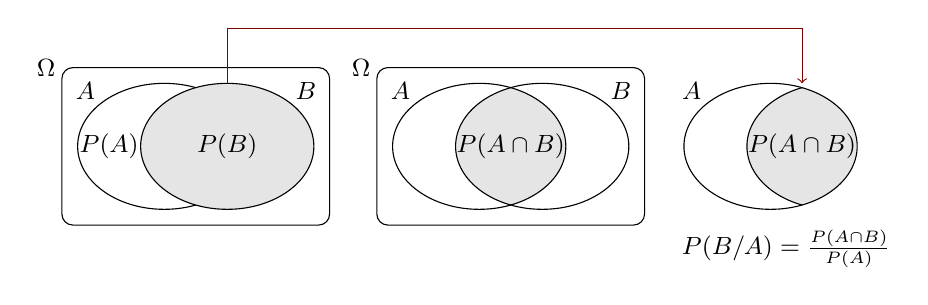
\begin{tikzpicture}[x=10mm,y=10mm,font=\small]

\def\rettangolo{-- ++(3.4,0) -- ++(0,2) -- ++(-3.4,0) -- cycle}
\def\insieme_int{-- ++(4,0) -- ++(0,3) -- ++(-4,0) -- cycle}
\def\firstcircle{(1.3,1) ellipse (1.1 and .8)}
\def\secondcircle{(2.1,1) ellipse (1.1 and .8)}
\def\thirdcircle{(5.3,1) ellipse (1.1 and .8)}
\def\fourthcircle{(6.1,1) ellipse (1.1 and .8)}
\def\fifthcircle{(9,1) ellipse (1.1 and .8)}
\def\sixthcircle{(9.8,1) ellipse (1.1 and .8)}
 %insieme1
\draw[rounded corners] (0,0) \rettangolo (-.2,2) node {$\Omega$};
\draw[->,color=Maroon] (2.1,1.8)--(2.1,2.5)--(9.4,2.5)--(9.4,1.8);
\draw \firstcircle (.6,1) node {$P(A)$} (.3,1.7) node {$A$};
\filldraw[fill=gray!20!,draw=black] \secondcircle node {$P(B)$} (3.1,1.7) node{$B$};

 \begin{scope}
     \clip \thirdcircle;
     \fill[color=gray!20!] \fourthcircle;
  \end{scope}

\draw \thirdcircle (4.3,1.7) node{$A$};
\draw \fourthcircle (5.7,1) node {$P(A \cap B)$}(7.1,1.7) node {$B$};
%insieme 2
\draw[rounded corners] (4,0) \rettangolo node at (3.8,2) {$\Omega$};
 \begin{scope}
     \clip \fifthcircle;
     \fill[color=gray!20!] \sixthcircle;
     \draw \sixthcircle (9.4,1) node {$P(A \cap B)$};
  \end{scope}

\draw \fifthcircle (8,1.7) node {$A$};
\draw (9.2,-.3) node {$P(B/A)=\frac{P(A \cap B)}{P(A)}$};
\end{tikzpicture}

\end{center}
Immaginiamo la misura della probabilità come una massa unitaria da spalmare 
sull'evento. La probabilità B è la quantità di massa da spalmare sull'evento B 
in relazione allo spazio degli eventi $\wp (\Omega )$. Nell'ipotesi di ricevere 
un'ulteriore informazione dal verificarsi di A, questa informazione modifica la 
probabilità di B. L'insieme di riferimento per la probabilità di B non sarà più 
$\wp (\Omega )$, ma $\wp (A)$ e $P(B/A)$ sarà data dal rapporto della massa 
spalmata tra ciò che hanno in comune A e B cioè $P(A\cap B)$ e la probabilità 
di 
A cioè $P(A)$: $P(B/A)=\frac{P(A\cap B)}{P(A)}$.

Se $P(B/A)=P(B)$ la parte della massa unitaria spalmata su B e il rapporto tra 
la massa spalmata sull'intersezione tra A e B e la massa spalmata su A rimane 
invariato e i due eventi si dicono indipendenti.

Se $P(B/A)>P(B)$ si dice che l'evento B è correlato positivamente all'evento A. 
Cioè il verificarsi di A aumenta la probabilità dell'evento B.

Se $P(B/A)<P(B)$ si dice che l'evento B è correlato negativamente all'evento A. 
Cioè il verificarsi di A diminuisce la probabilità dell'evento B.
\osservazione Due eventi A e B tra loro incompatibili cioè tali che $P(A\cap 
B)=0$ sono fortemente dipendenti. Infatti 
\[P(B/A)=\frac{P(A\cap B)}{P(A)}=\frac 0{P(A)}=0\neq P(B).\]

In genere $ P(A/B)\neq P(B/A) $ in quanto le due probabilità pur avendo lo 
stesso numeratore hanno quasi sempre denominatore diverso: 
\[P(B/A)=\frac{P(A\cap B)}{P(A)}\neq P(A/B)=\frac{P(A\cap B)}{P(B)}.\]

Per la proprietà commutativa della intersezione abbiamo: $P(A\cap B)=P(B\cap 
A)$ 
quindi 
\[P(A\cap B)=P(A)\cdot P(B/A)=P(B)\cdot P(A/B).\]

% \begin{exrig}
\begin{esempio}
Conviene scommettere alla pari che in una classe composta da 23 alunni, due 
persone compiano gli anni nello stesso giorno dello stesso mese?

In questo esempio non consideriamo gli anni bisestili e che la probabilità di 
nascere in un giorno dell'anno sia la stessa per tutti i giorni dell'anno. 
Scommettere alla pari significa intanto attribuire alla probabilità dell'evento 
A il valore di 0,5. Se la probabilità dell'evento è maggiore di 0,5 conviene 
scommettere altrimenti no.

Anche in questo caso conviene calcolare la probabilità dell'evento 
complementare 
$P(\overline A)$ cioè la probabilità che nessuno dei 23 allievi compiano gli 
anni nello stesso giorno dello stesso mese.
\[P(\overline A)=P(\overline A_1\cap 
\overline A_2\cap \overline A_2\ldots \overline A_{21}\cap \overline A_{22}\cap 
\overline A_{23})\] dove $\overline{A_i}$ rappresenta la probabilità che il 
compleanno dell'alunno \emph{i}{}-esimo non coincida con nessuno dei compleanni 
degli altri alunni.

Analizziamo alcune di queste probabilità e applichiamo il teorema delle 
probabilità composte: \[P(\overline A_1)=\frac{365}{365}\quad ;\quad \ P(\overline 
A_2/\overline A_1)=\frac{364}{365} \quad ;\quad  P(\overline A_3/\overline A_1\cap 
\overline 
A_2)=\frac{363}{365}\quad ;\quad \dots\] e così via fino ad arrivare a: 
\[P(\overline A_{23}/\overline A_1\cap \overline A_2\cap \overline A_2\ldots 
\overline A_{21}\cap \overline A_{22})=\frac{343}{365}\]

Il primo allievo avrà la certezza di non avere alcun allievo che compie gli 
anni 
nello stesso suo giorno; il secondo allievo avrà una probabilità pari a 364 
giorni su 365 di non compiere gli anni nello stesso giorno del primo, il terzo 
allievo una probabilità di 363 giorni su 365 condizionata a non compiere gli 
anni lo stesso giorno del primo e del secondo e così via fino alla probabilità 
dell'ultimo allievo pari a 343 giorni su 365 di non compiere gli anni lo stesso 
giorno dei propri compagni.

Ora applichiamo il teorema delle probabilità composte: \[ P(\overline 
A)=\frac{365}{365}\cdot \frac{364}{365}\cdot \frac{363}{365}\cdot 
\frac{362}{365}\ldots \cdot \frac{345}{365}\cdot \frac{344}{365}\cdot 
\frac{343}{365}=\frac{365\cdot 364\cdot 363\ldots 345 \cdot 344\cdot 
343}{365^{23}}=0,493. \] Dato che $P(A)=1-P(\overline A)=1-0,493=0,507$.
\conclusione Conviene scommettere alla pari sull'evento $ A $.
\end{esempio}
% \end{exrig}
Il problema dell'esempio precedente si può così schematizzare: in un'urna ci 
sono $ 365 $ palline numerate da $ 1 $ a $ 365 $, qual'è la probabilità, 
rimettendo la pallina nell'urna, di estrarre la stessa pallina in 23 estrazioni?

% \vspazio\ovalbox{\risolvii \ref{ese:9.60}, \ref{ese:9.61}, \ref{ese:9.62}, 
% \ref{ese:9.63}, \ref{ese:9.64}.}
